\documentclass[aspectratio=169,10pt]{beamer}

\usetheme{Madrid}
\usecolortheme{default}
\setbeamertemplate{navigation symbols}{}
\setbeamertemplate{footline}[frame number]
\setbeamertemplate{bibliography item}[text]

\usepackage{amsmath,amssymb,booktabs,array,graphicx,tikz}
\usepackage{appendixnumberbeamer}
\usetikzlibrary{arrows.meta,positioning,calc}
\pdfstringdefDisableCommands{\def\translate#1{#1}}

\definecolor{nbblue}{HTML}{0173B2}
\definecolor{nborange}{HTML}{DE8F05}
\definecolor{nbgreen}{HTML}{029E73}
\definecolor{nbred}{HTML}{B00020}
\definecolor{nbgray}{HTML}{5B6573}
\setbeamercolor{structure}{fg=nbblue}
\setbeamercolor{title}{fg=nbblue}
\setbeamercolor{frametitle}{fg=white,bg=nbblue}
\setbeamercolor{alerted text}{fg=nborange}

\graphicspath{{../analysis/report_figures/}}
\newcommand{\pct}{\,\%}
\newcommand{\takeaway}[1]{%
  \vspace{0.3em}\begin{beamercolorbox}[rounded=true,sep=0.55em]{block body}
  \textbf{#1}
  \end{beamercolorbox}}
\newcommand{\todobox}[1]{%
  \begin{beamercolorbox}[rounded=true,sep=0.55em,wd=\linewidth]{alerted text}
  \centering\color{nbred}\bfseries\Large TODO\normalsize\quad #1
  \end{beamercolorbox}}

\title{Monthly meeting\\26/08/2026}
\author{Philippe Forest}
\institute{IMT Atlantique}
\date{}

\begin{document}

\begin{frame}[plain]
  \centering
  \vfill
  {\color{nbblue}\bfseries\fontsize{24}{28}\selectfont
    Monthly meeting\\[0.2em]26/08/2026}

  \vspace{1.2em}
  {\large Philippe Forest}

  \vspace{0.25em}
  {\small IMT Atlantique}

  \vfill
\end{frame}

\section{Setup}

\begin{frame}{Evaluation protocol}
  \begin{columns}[T,onlytextwidth]
    \column{0.49\textwidth}
      \textbf{Each member}
      \begin{itemize}
        \item 50 epochs, pairwise subject mixup
        \item checkpoint selected on held-out test loss unless stated
        \item plain cosine retrieval; no transductive adaptation
      \end{itemize}

    \column{0.49\textwidth}
      \textbf{Fixed ensemble rule}
      \[
        z_m(q,c)=\frac{s_m(q,c)-\mu_m(q)}{\sigma_m(q)},
        \qquad
        s_{\mathrm{ens}}=\frac{1}{k}\sum_{m=1}^{k}z_m .
      \]
      For each EEG trial, standardize every model's 200 candidate scores,
      then average corresponding candidates and select the highest score.
  \end{columns}
\end{frame}

\section{Where the gains come from}

\begin{frame}{Seed diversity}
  \centering
  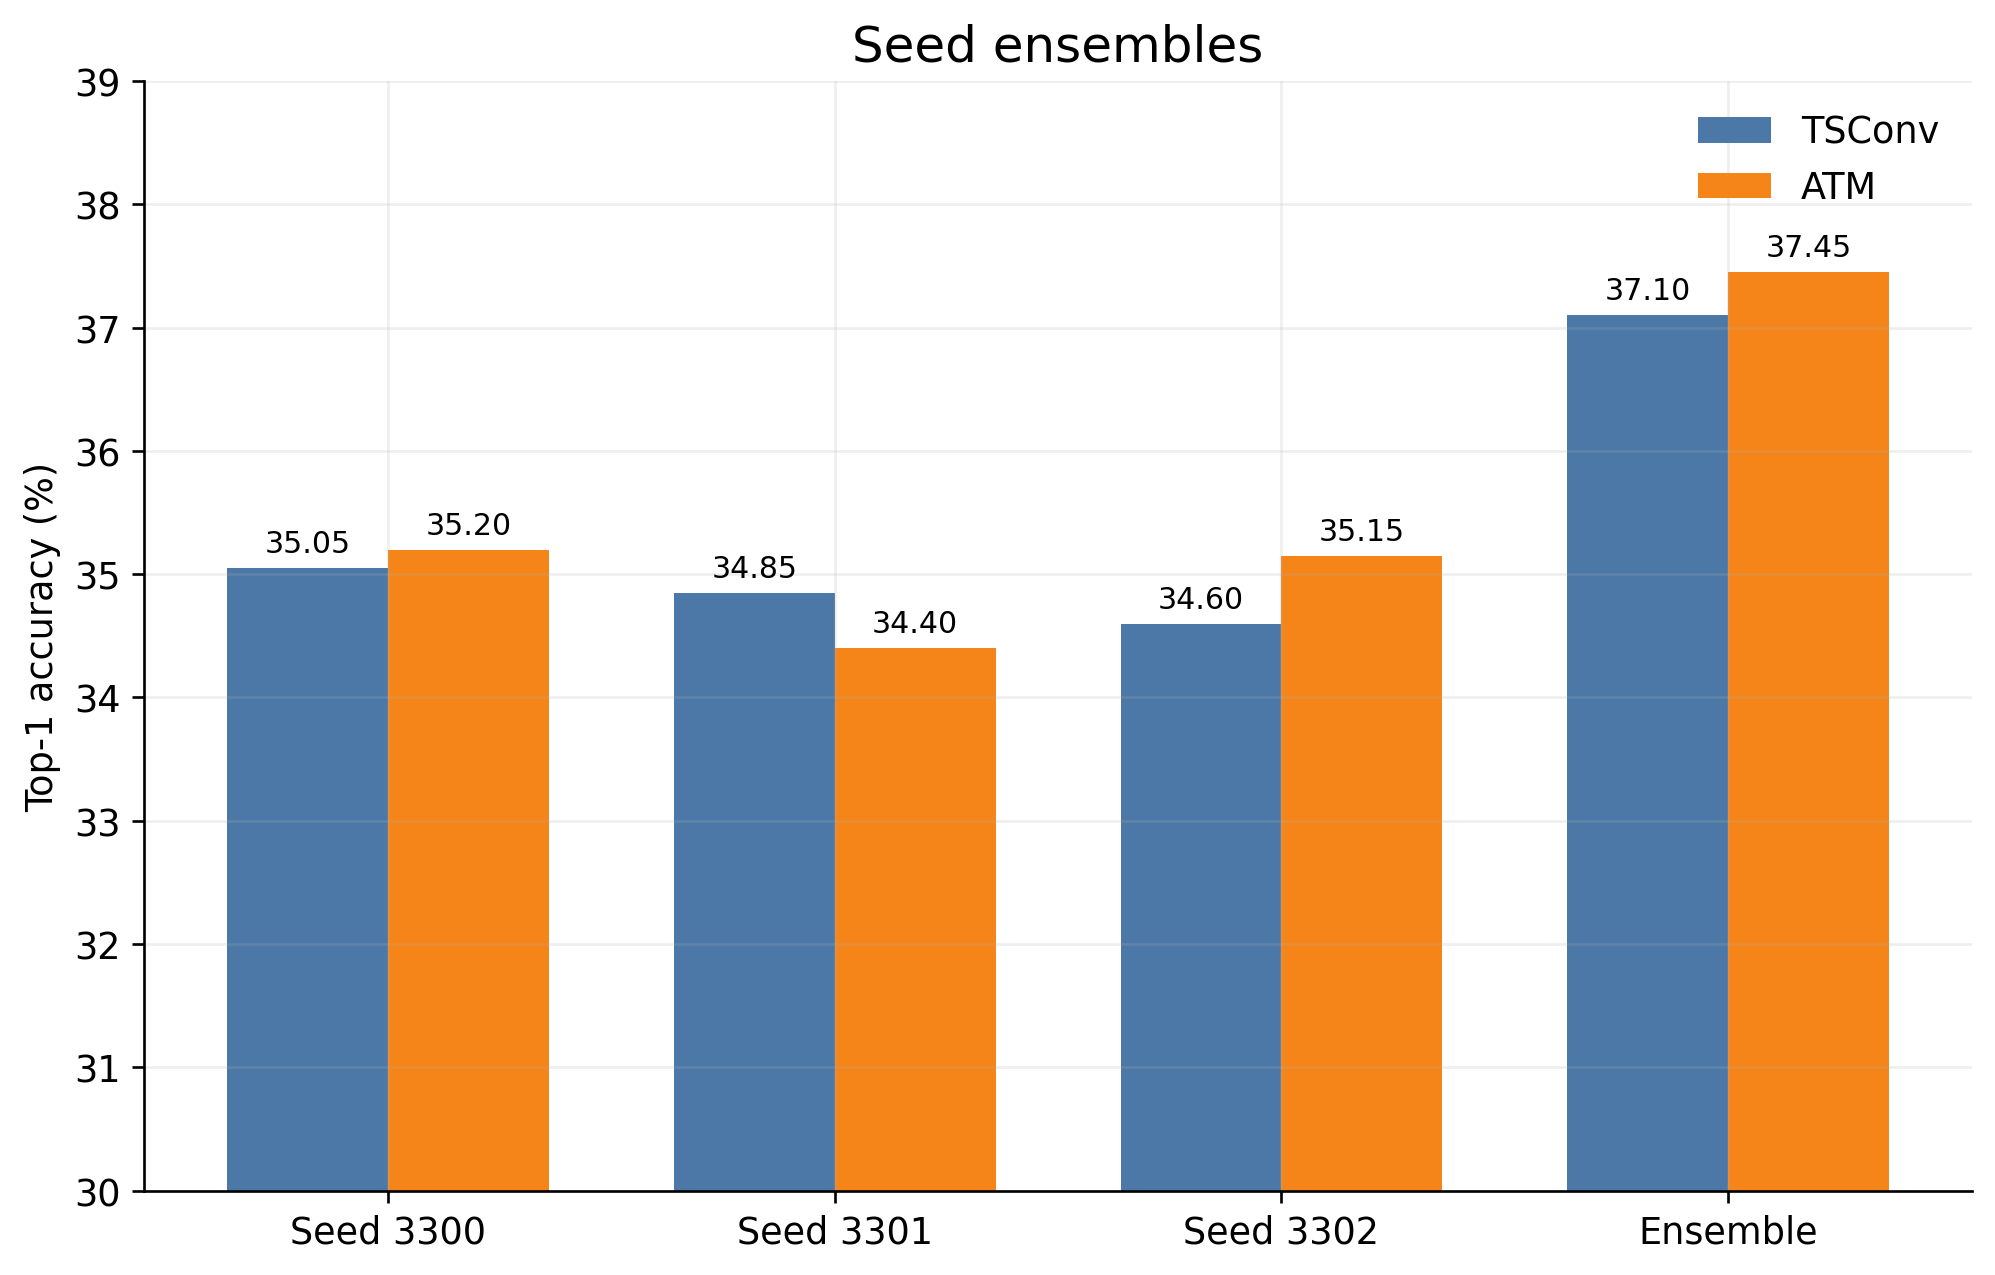
\includegraphics[width=0.87\textwidth,height=0.69\textheight,keepaspectratio]{seed_ensembles.png}

  \small TSConv and ATM are the two strongest EEG encoders for this task,
  but use distinct inductive biases: temporal--spatial convolution versus attention-based token mixing.
\end{frame}

\begin{frame}{Image-depth diversity protocol}
  \begin{columns}[T,onlytextwidth]
    \column{0.46\textwidth}
      \textbf{Reference condition}
      \begin{itemize}
        \item one EEG encoder per LOSO fold
        \item target: intermediate InternViT layer 28
        \item same 50-epoch training and row-z fusion
      \end{itemize}

    \column{0.49\textwidth}
      \textbf{Depth intervention}
      \begin{itemize}
        \item retain the EEG architecture and training recipe
        \item align separate models to layers 23, 25, 28, 31, 33, and 35
        \item ensemble models trained toward different visual abstractions
      \end{itemize}
  \end{columns}

  \vspace{1.0em}
  \centering
  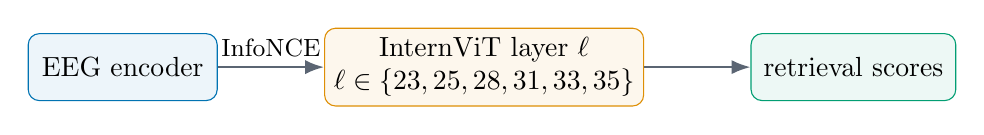
\begin{tikzpicture}[
      box/.style={draw,rounded corners,minimum height=0.85cm,align=center},
      arr/.style={-{Latex[length=2.4mm]},thick,draw=nbgray}]
    \node[box,draw=nbblue,fill=nbblue!7,minimum width=2.4cm] (eeg) {EEG encoder};
    \node[box,draw=nborange,fill=nborange!7,minimum width=3.2cm,right=1.35cm of eeg] (target)
      {InternViT layer $\ell$\\$\ell\in\{23,25,28,31,33,35\}$};
    \node[box,draw=nbgreen,fill=nbgreen!7,minimum width=2.6cm,right=1.35cm of target] (score)
      {retrieval scores};
    \draw[arr] (eeg) -- node[above,font=\small] {InfoNCE} (target);
    \draw[arr] (target) -- (score);
  \end{tikzpicture}

\end{frame}

\begin{frame}{Image-depth diversity}
  \centering
  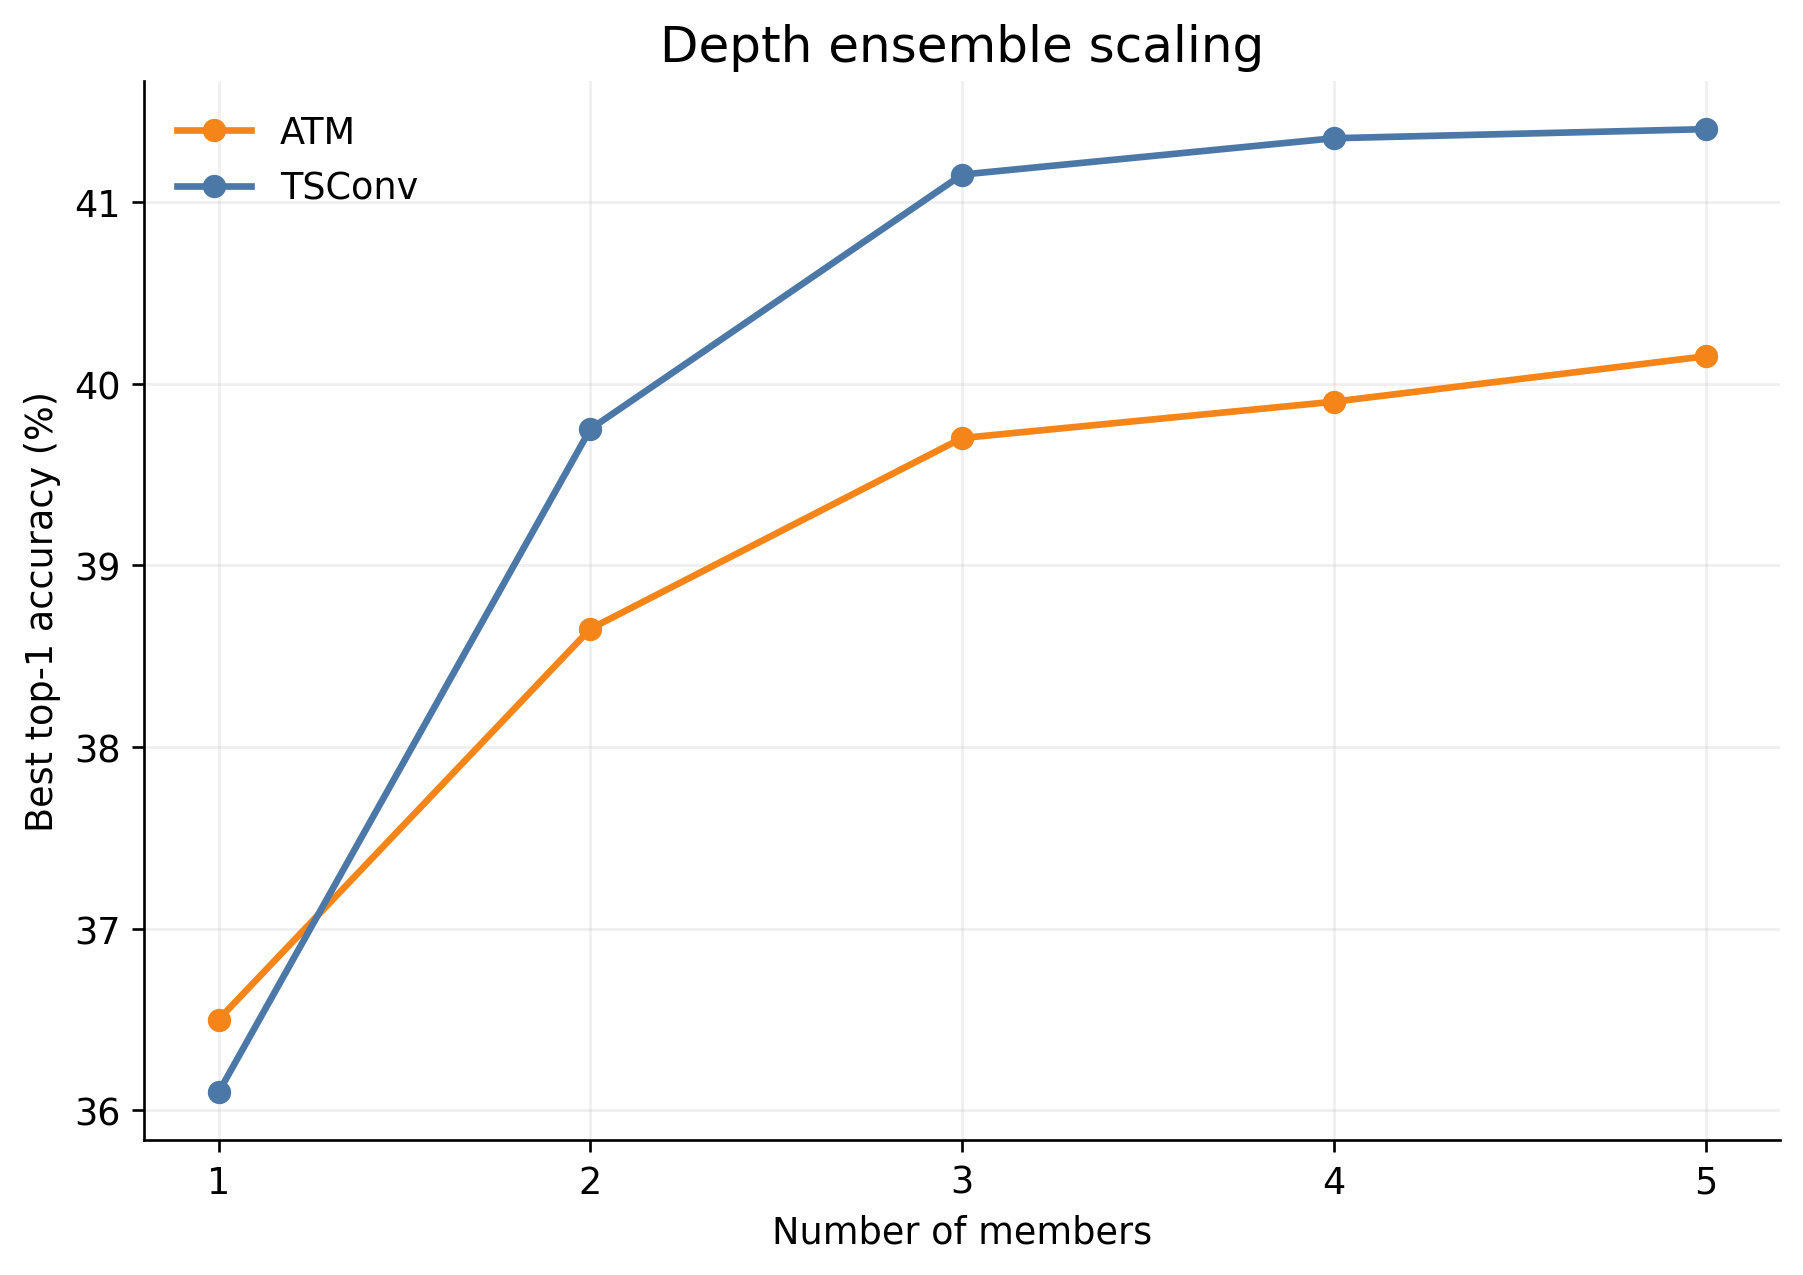
\includegraphics[width=0.90\textwidth,height=0.72\textheight,keepaspectratio]{depth_ensemble_scaling.png}

  \takeaway{Depth changes help, but same-family committees saturate near $40$--$41\pct$.}
\end{frame}

\begin{frame}{ATM + TSConv}
  \centering
  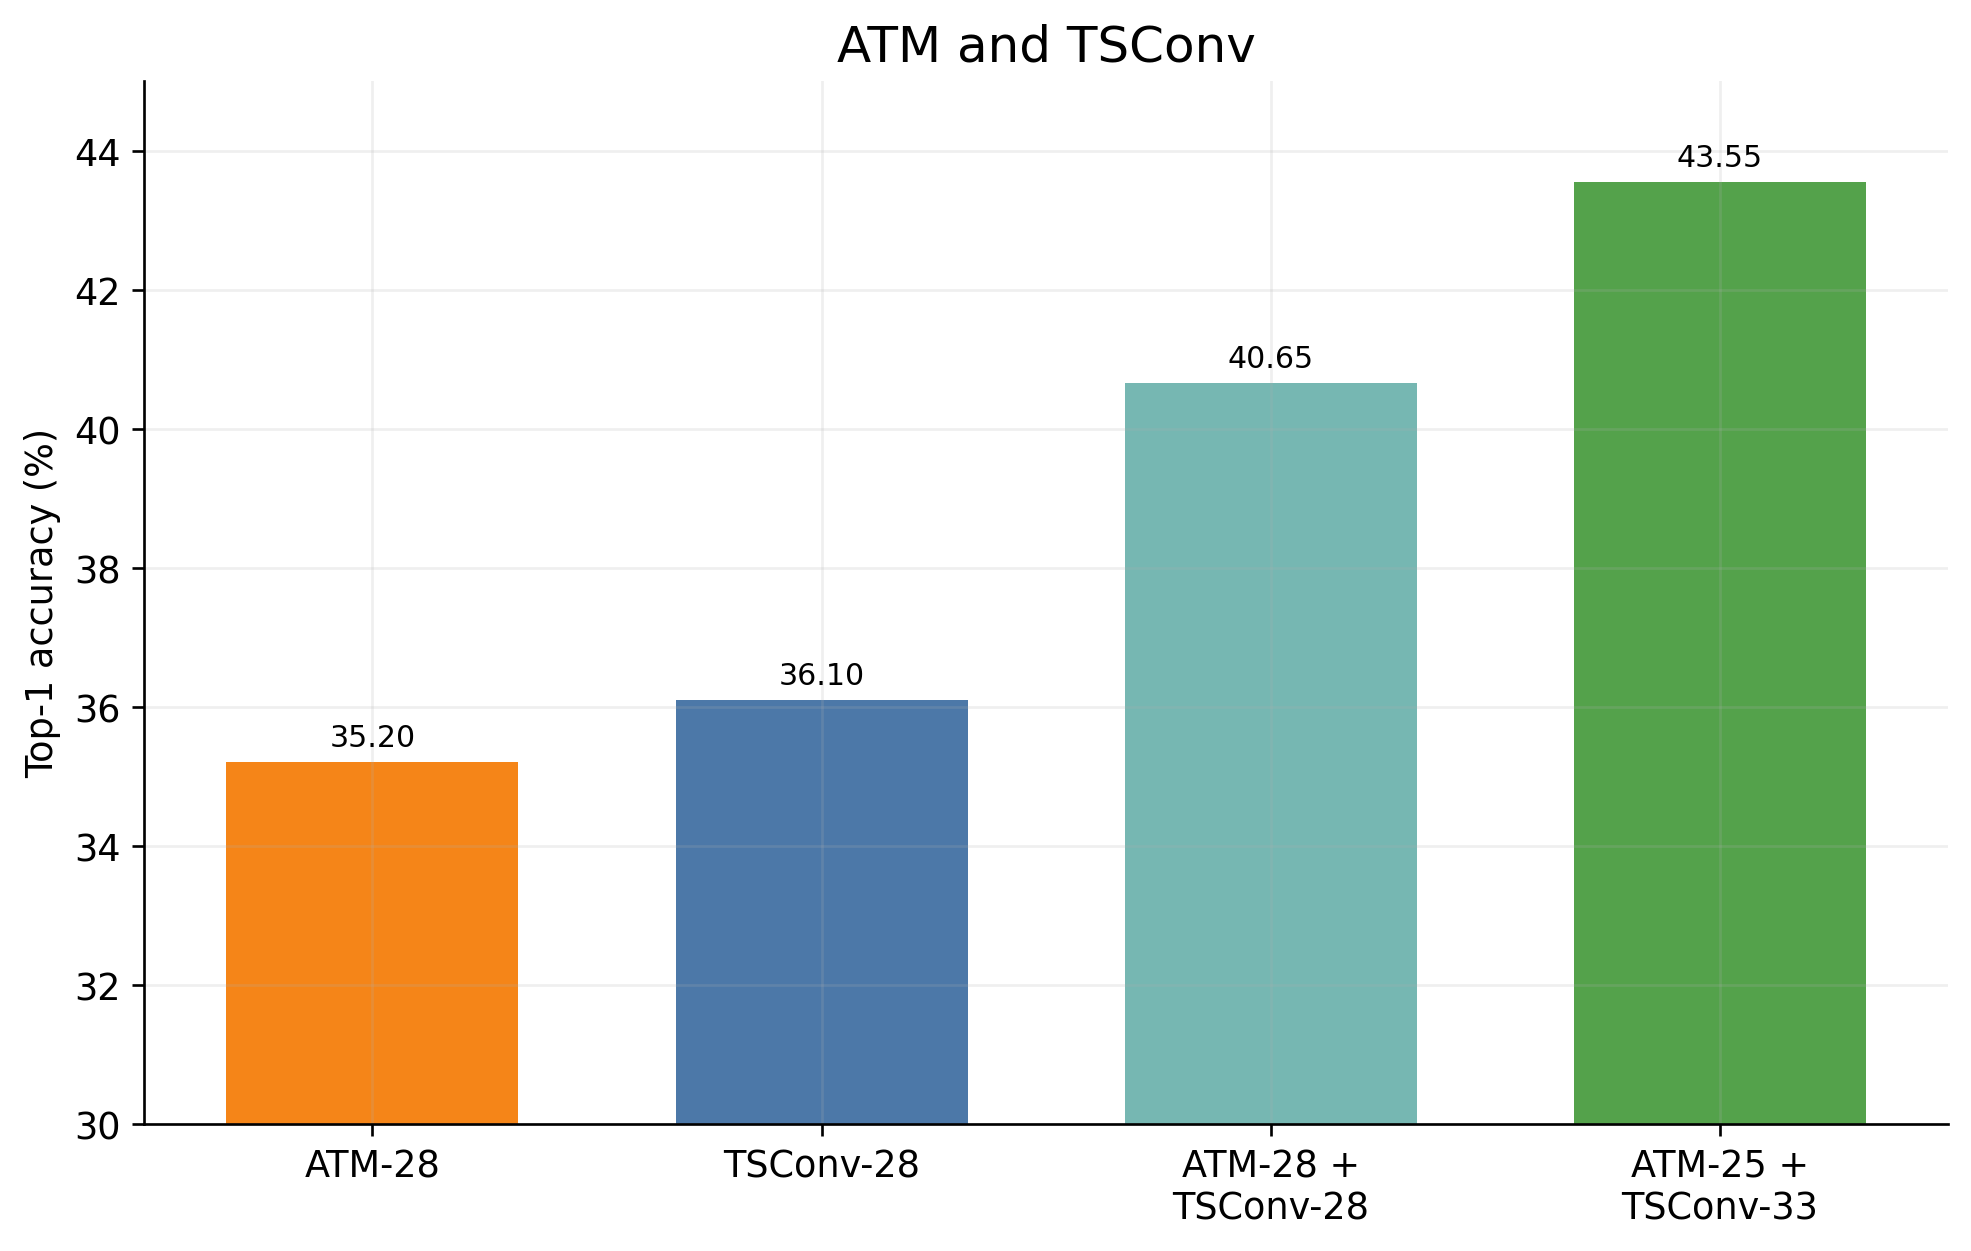
\includegraphics[width=0.86\textwidth,height=0.70\textheight,keepaspectratio]{atm_tsconv_pair.png}

  \takeaway{Changing both encoder and visual depth reaches $43.55\pct$, versus $40.65\pct$ at layer 28.}
\end{frame}


\begin{frame}{The compact four-member committee}
  \small We pooled every compatible trained model in the repository and greedily added
  the member that maximized all-ten row-z accuracy at each step.

  \vspace{0.45em}
  \begin{columns}[T,onlytextwidth]
    \column{0.43\textwidth}
      \textbf{Best $k=4$: $48.20\pct$}

      \smallskip
      \textbf{Model (visual target)}
      \begin{itemize}
        \item Squeezeformer (InternViT-28)
        \item ATM (ViT-H)
        \item ATM (InternViT-28 group)
        \item TSConv (InternViT-33 group)
      \end{itemize}
      Removing any member costs $2.55$--$3.45$ points.

    \column{0.55\textwidth}
      \centering
      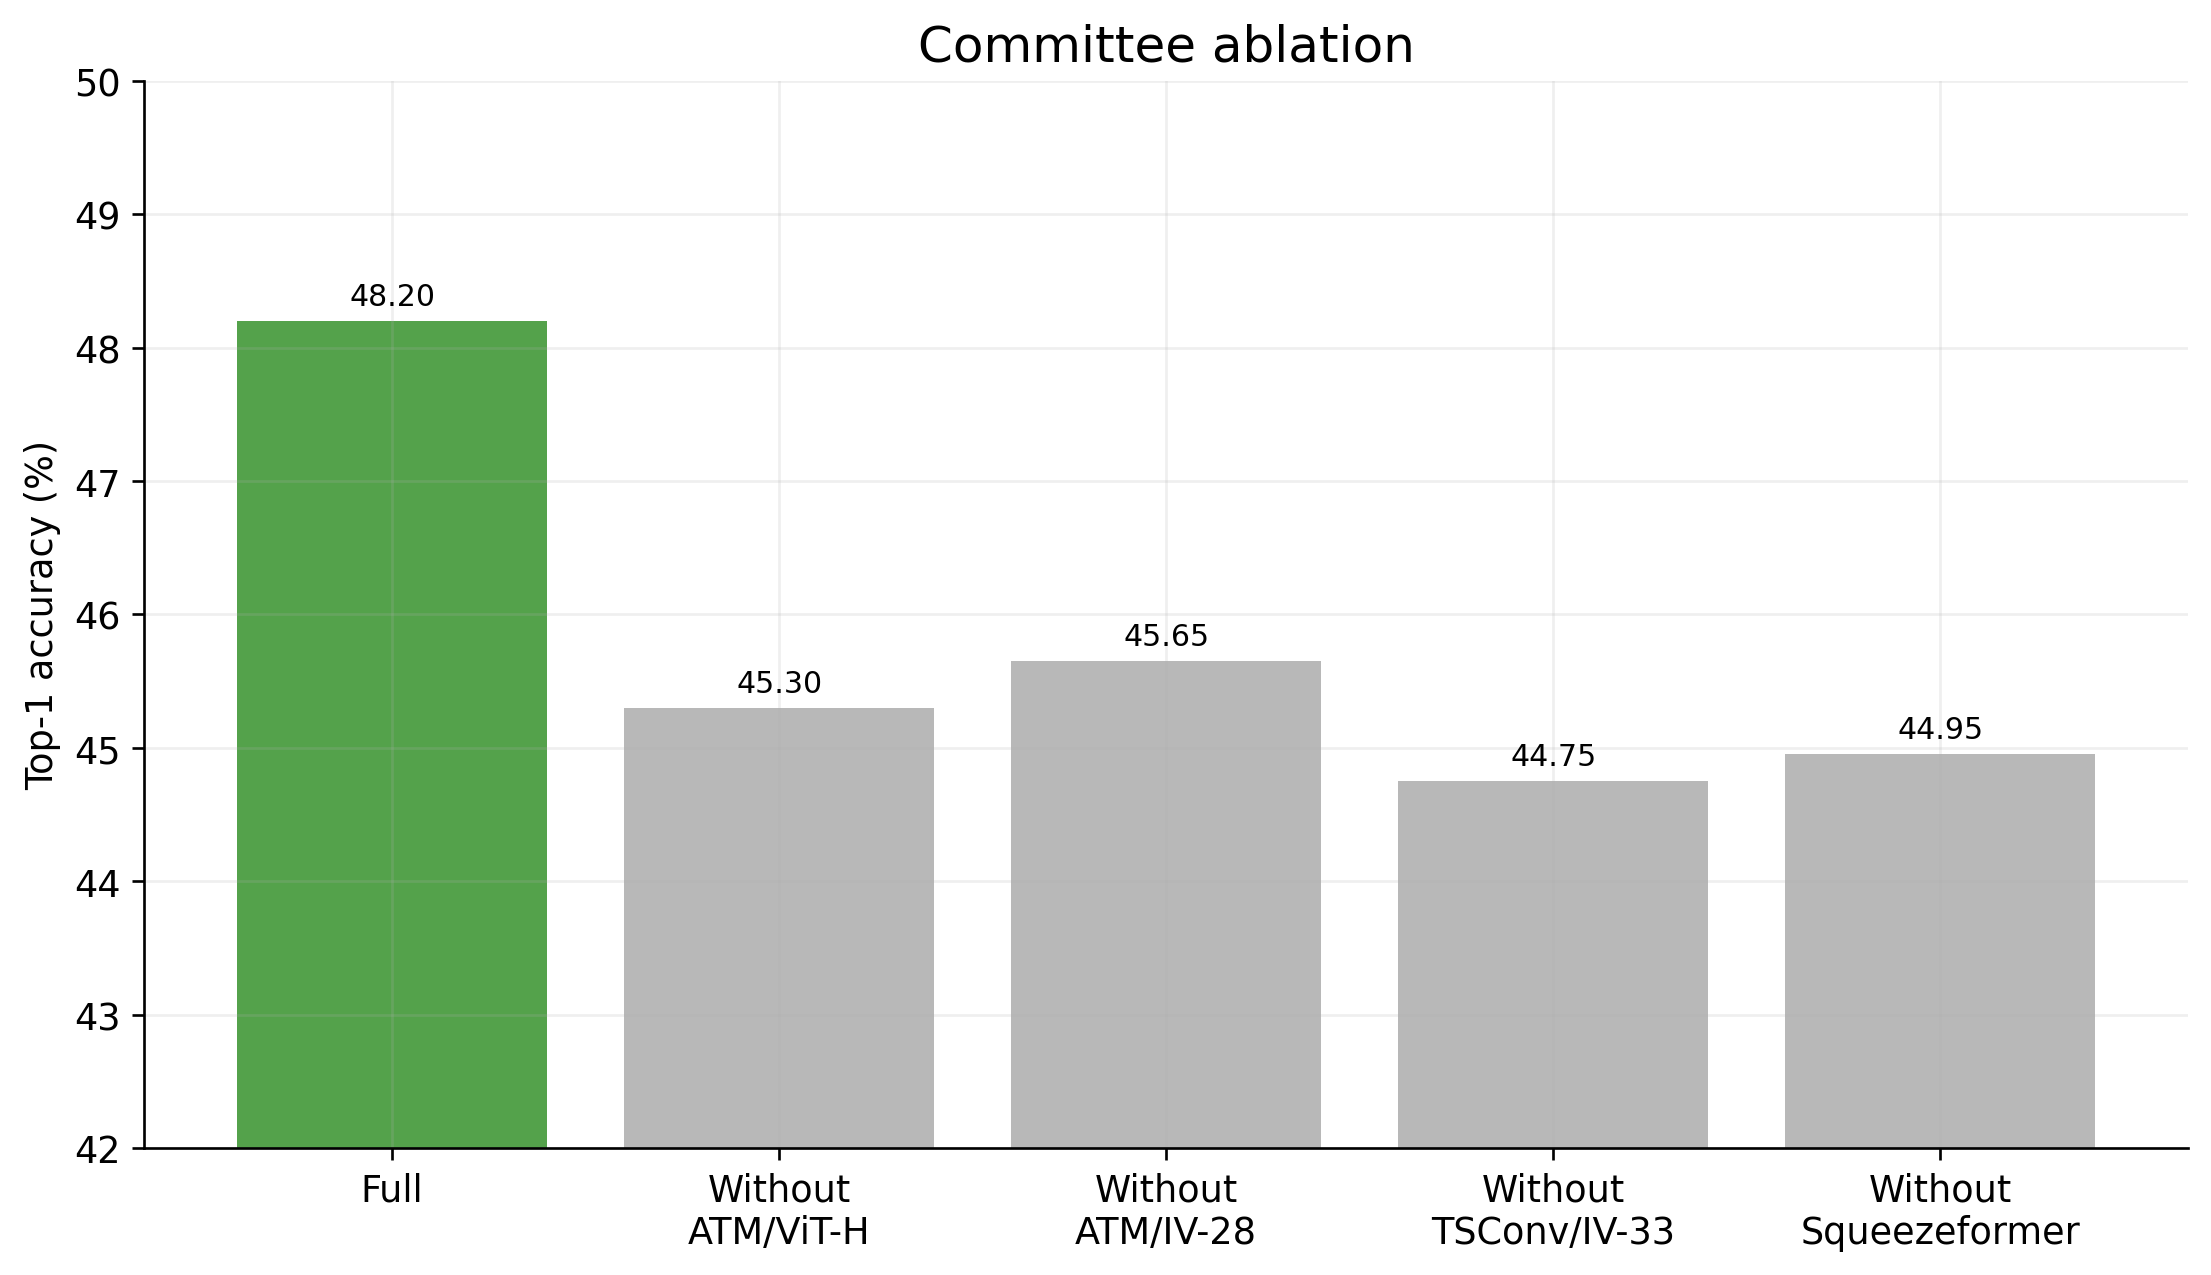
\includegraphics[width=\linewidth,height=0.67\textheight,keepaspectratio]{committee_ablation.png}
  \end{columns}
\end{frame}

{\setbeamertemplate{footline}{}
\begin{frame}{Ensemble scaling}
  \centering
  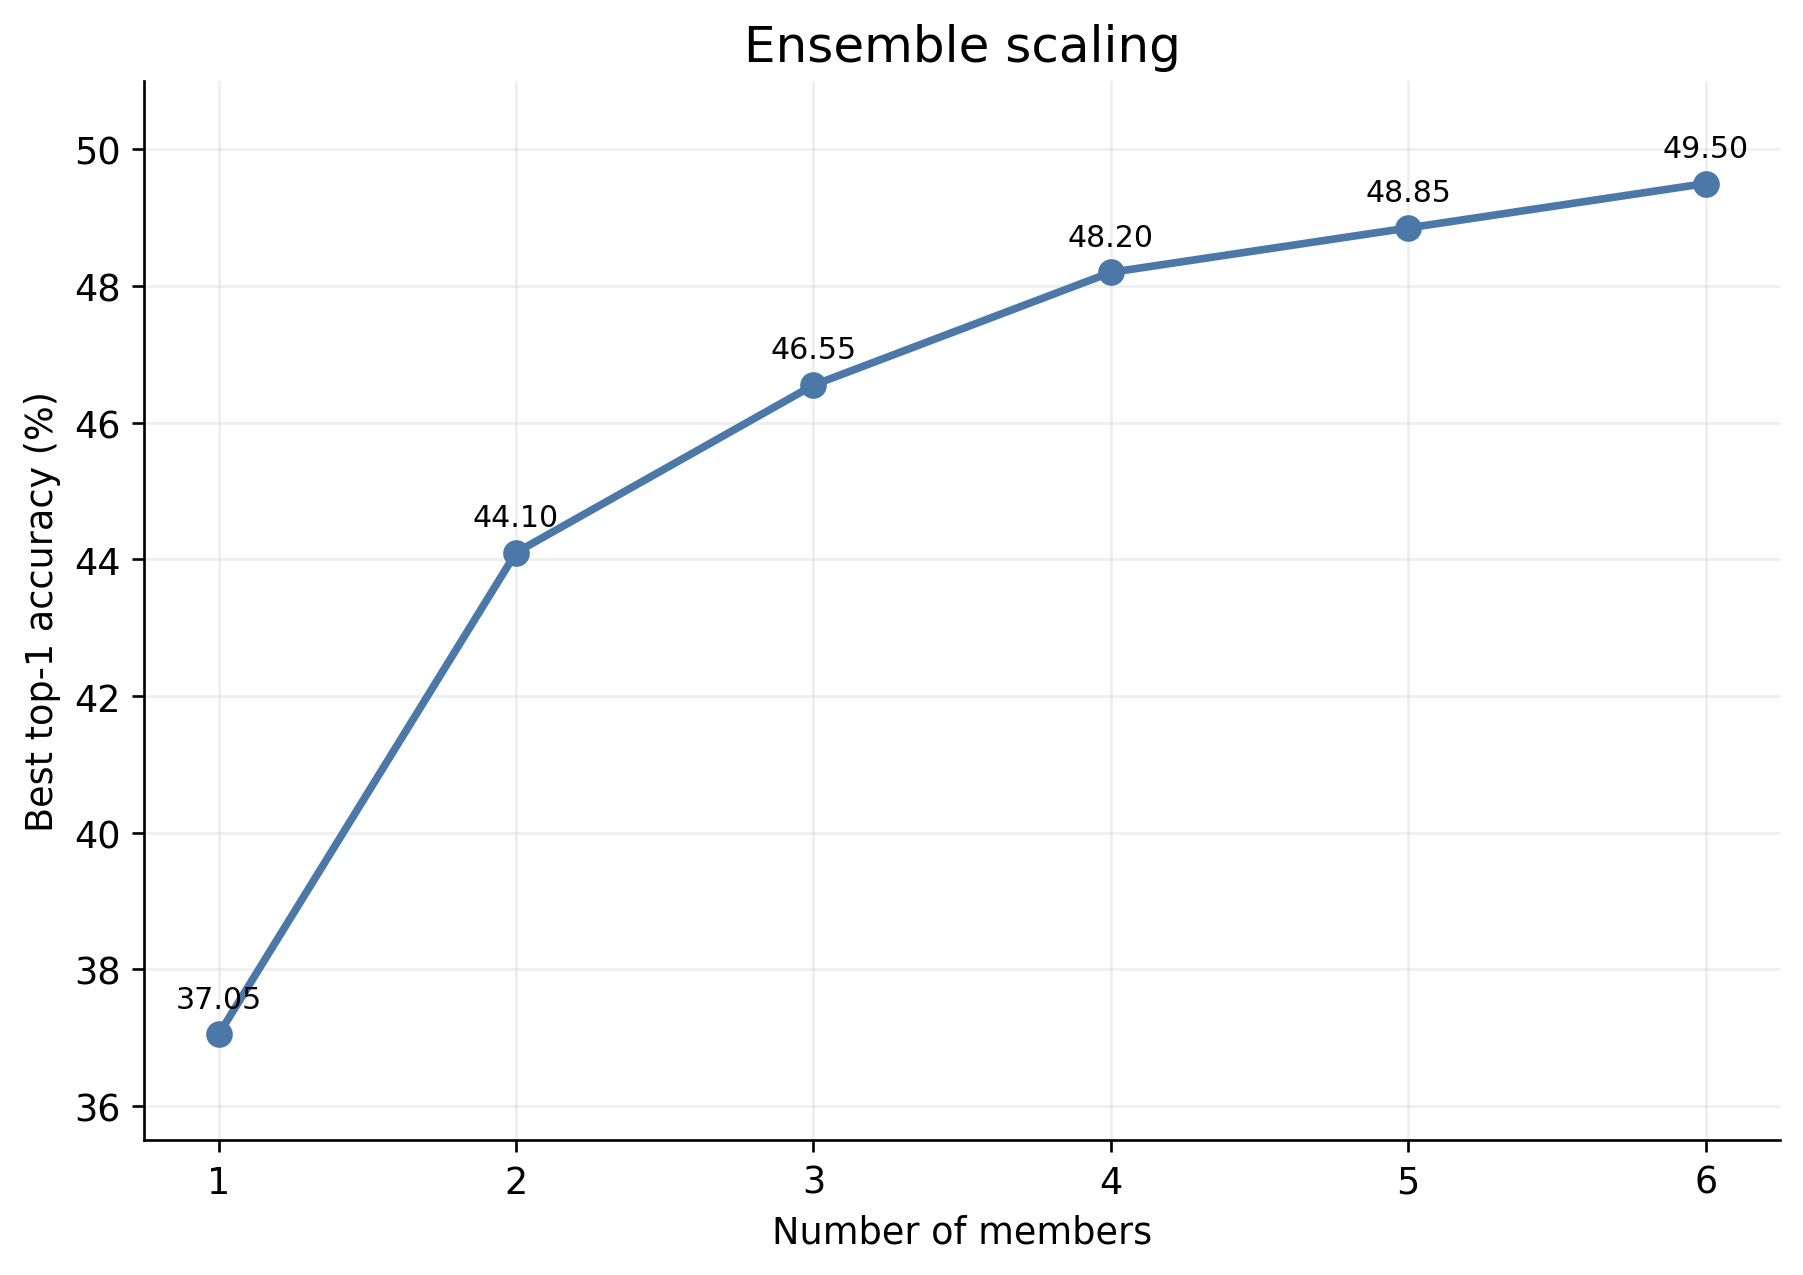
\includegraphics[width=0.90\textwidth,height=0.79\textheight,keepaspectratio]{ensemble_scaling.png}
\end{frame}
}

\begin{frame}{Cross-subject retrieval state of the art}

  \centering
  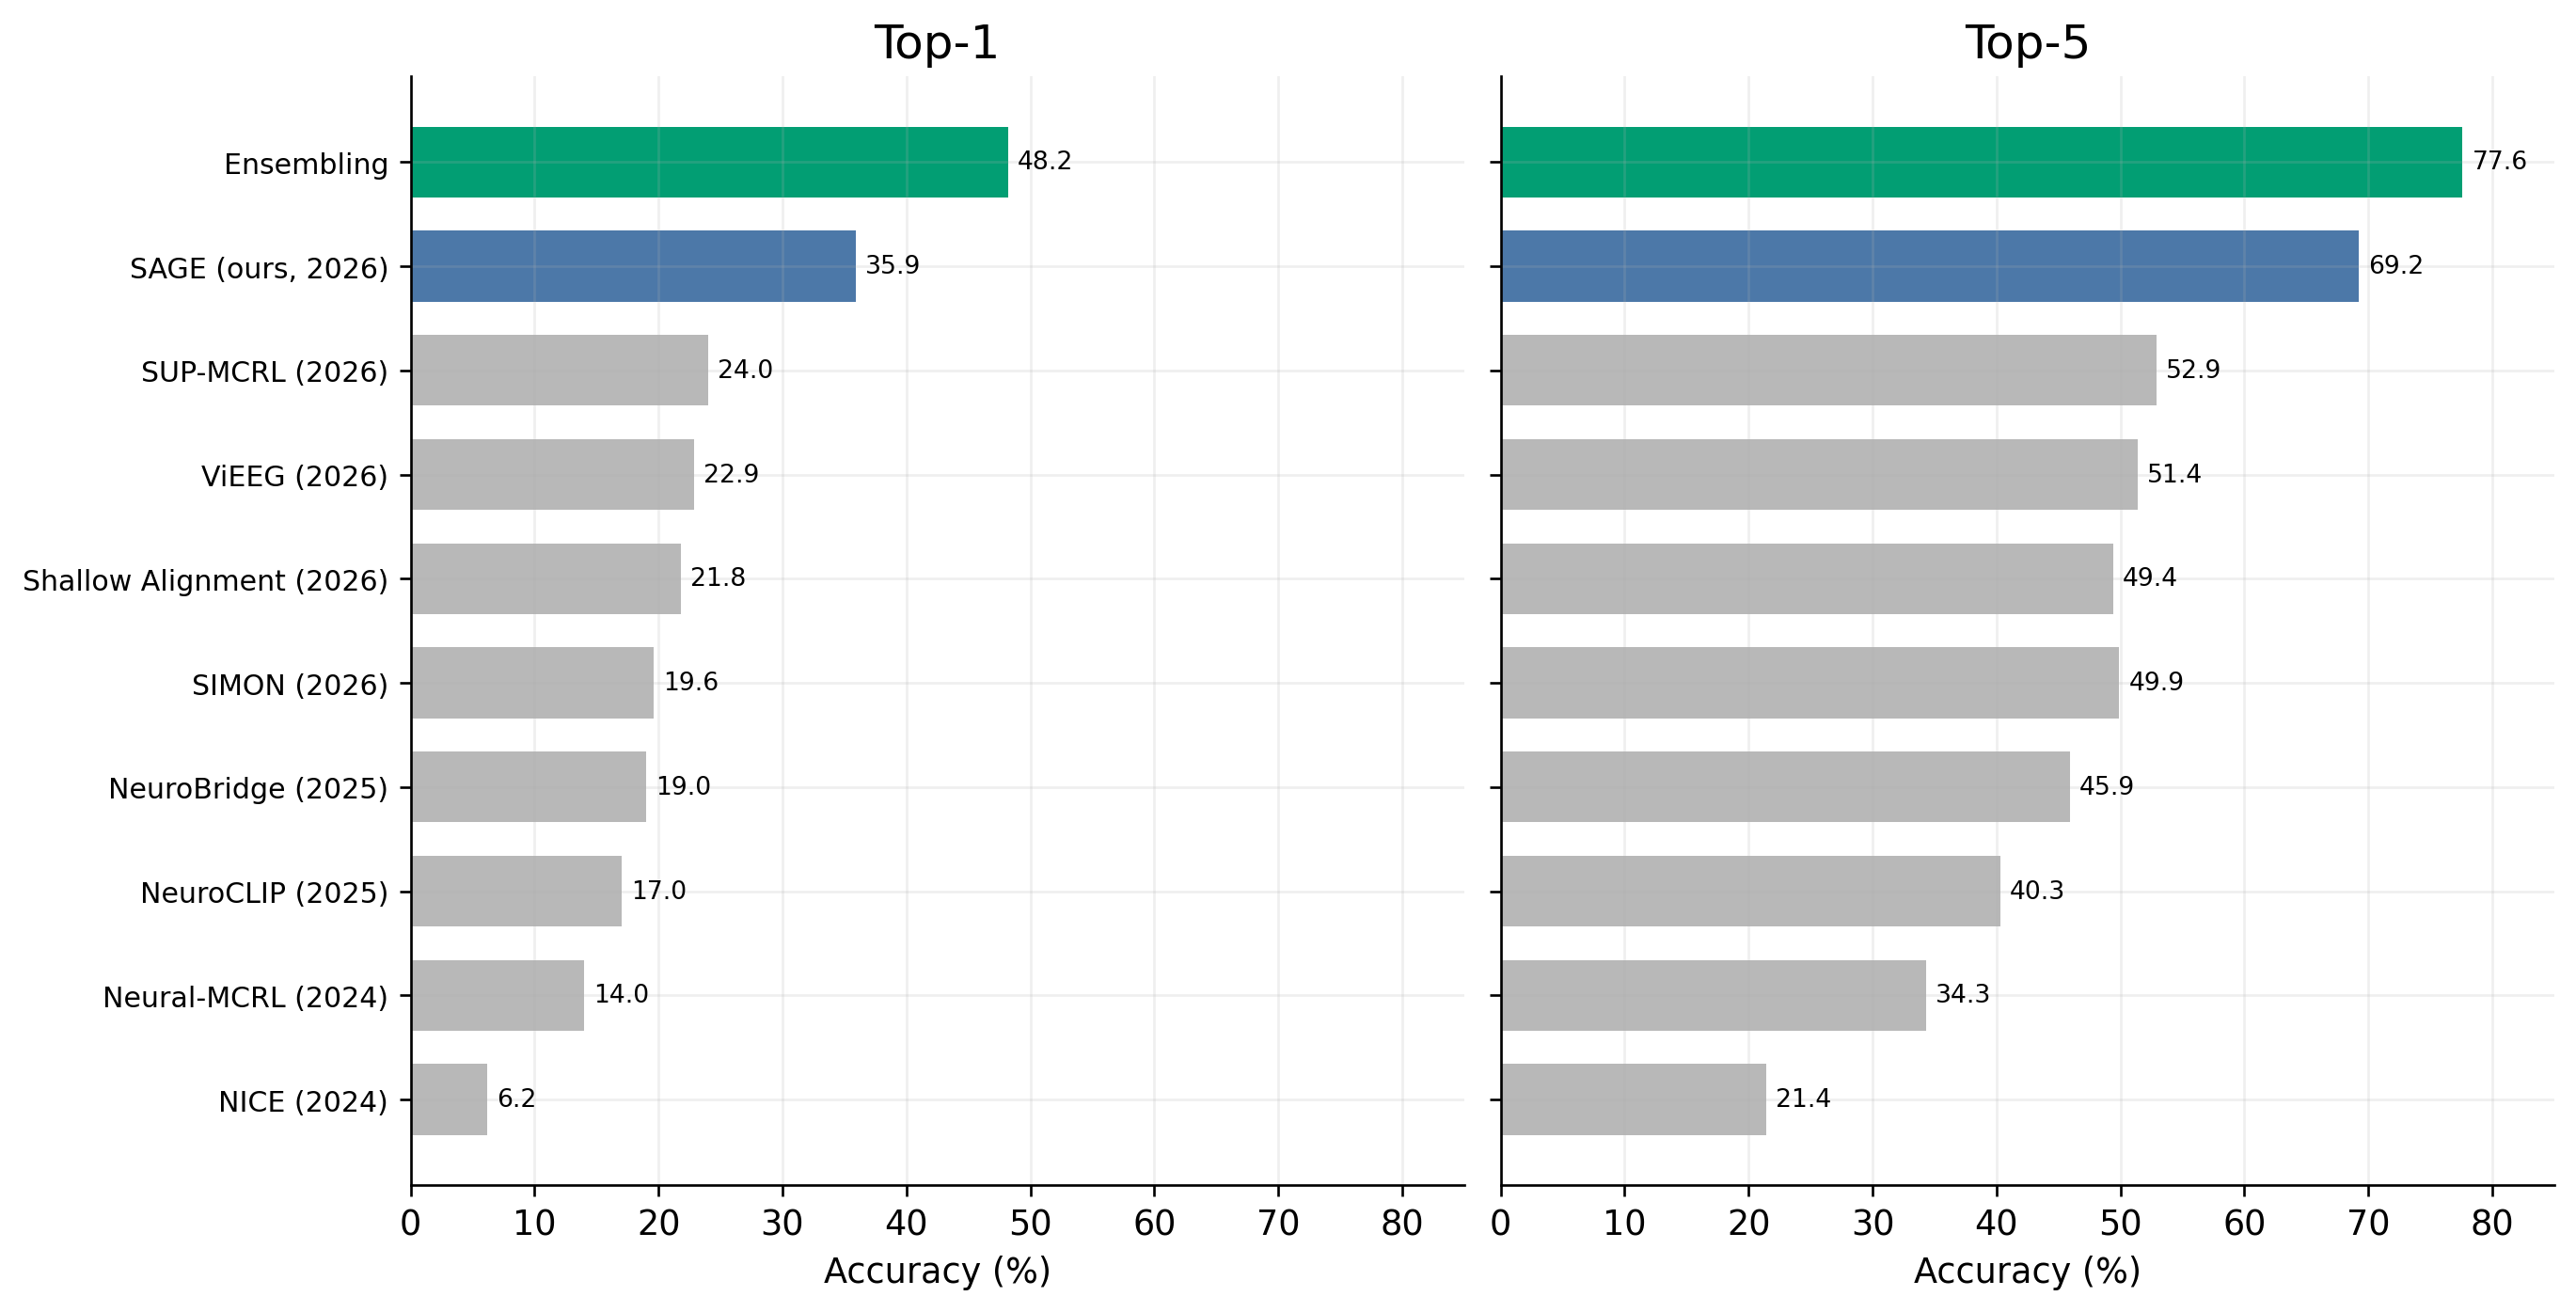
\includegraphics[width=0.93\textwidth,height=0.66\textheight,keepaspectratio]{sota_comparison.png}

  \textbf{Ensembling reaches $48.20\pct$ top-1 and $77.60\pct$ top-5, well above the current SOTA.}
\end{frame}

\begin{frame}{Decorrelation drives gains}
  \centering
  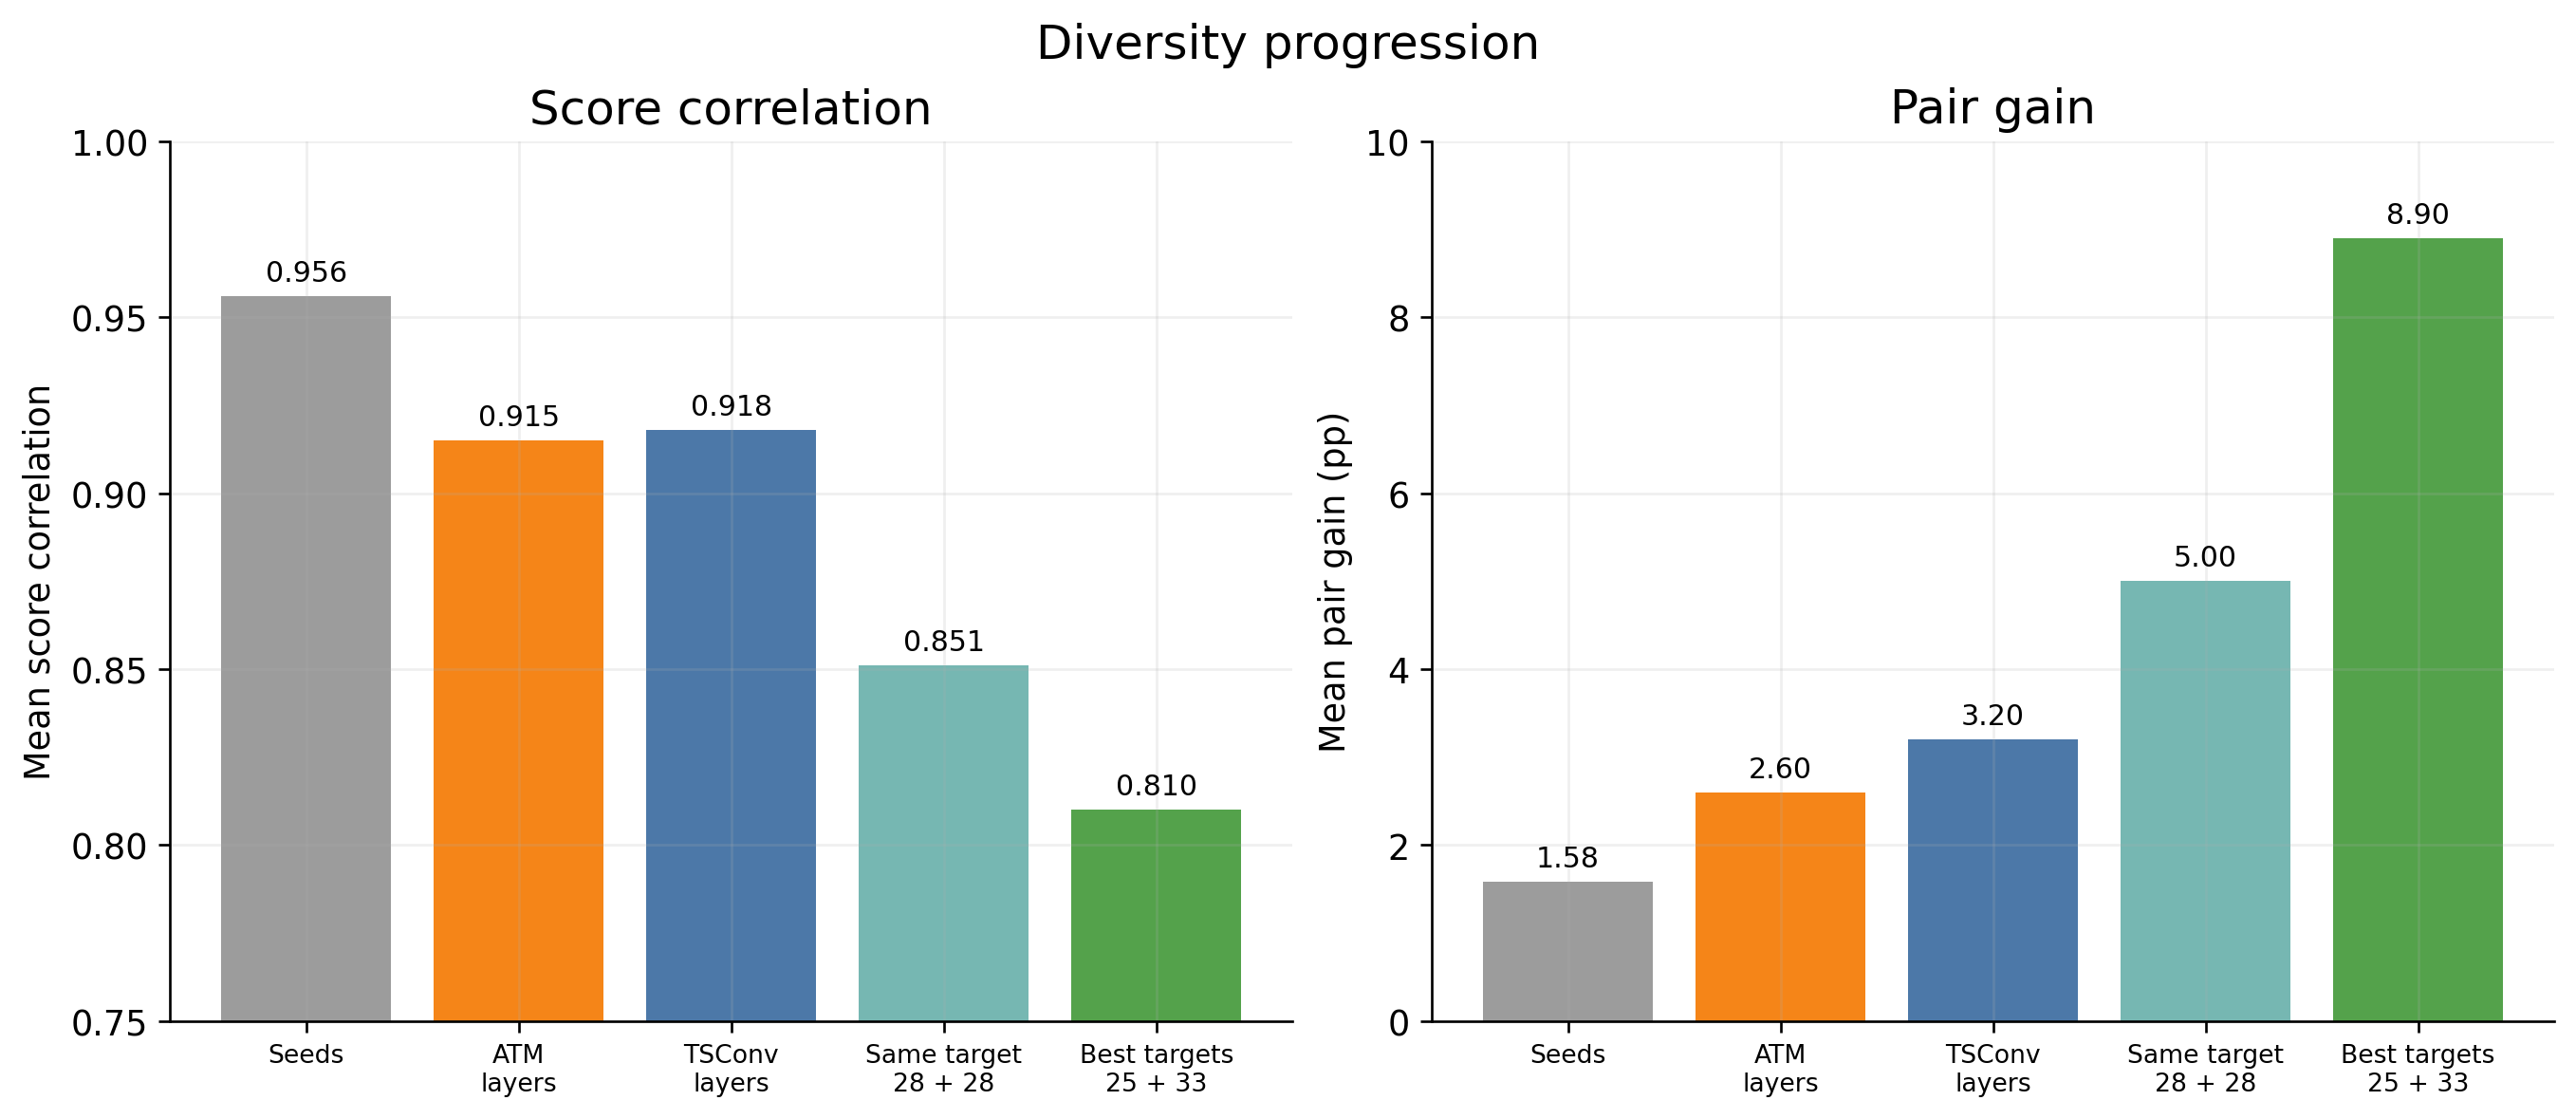
\includegraphics[width=0.92\textwidth,height=0.68\textheight,keepaspectratio]{diversity_progression.png}

  \vspace{0.2em}
  \small \textbf{Score correlation:} Pearson correlation between two models' row-z-normalized
  200-way score vectors, pooled over every trial and LOSO fold.
\end{frame}

\section{What predicts complementarity?}

\begin{frame}{Pairwise complementarity}
  \centering
  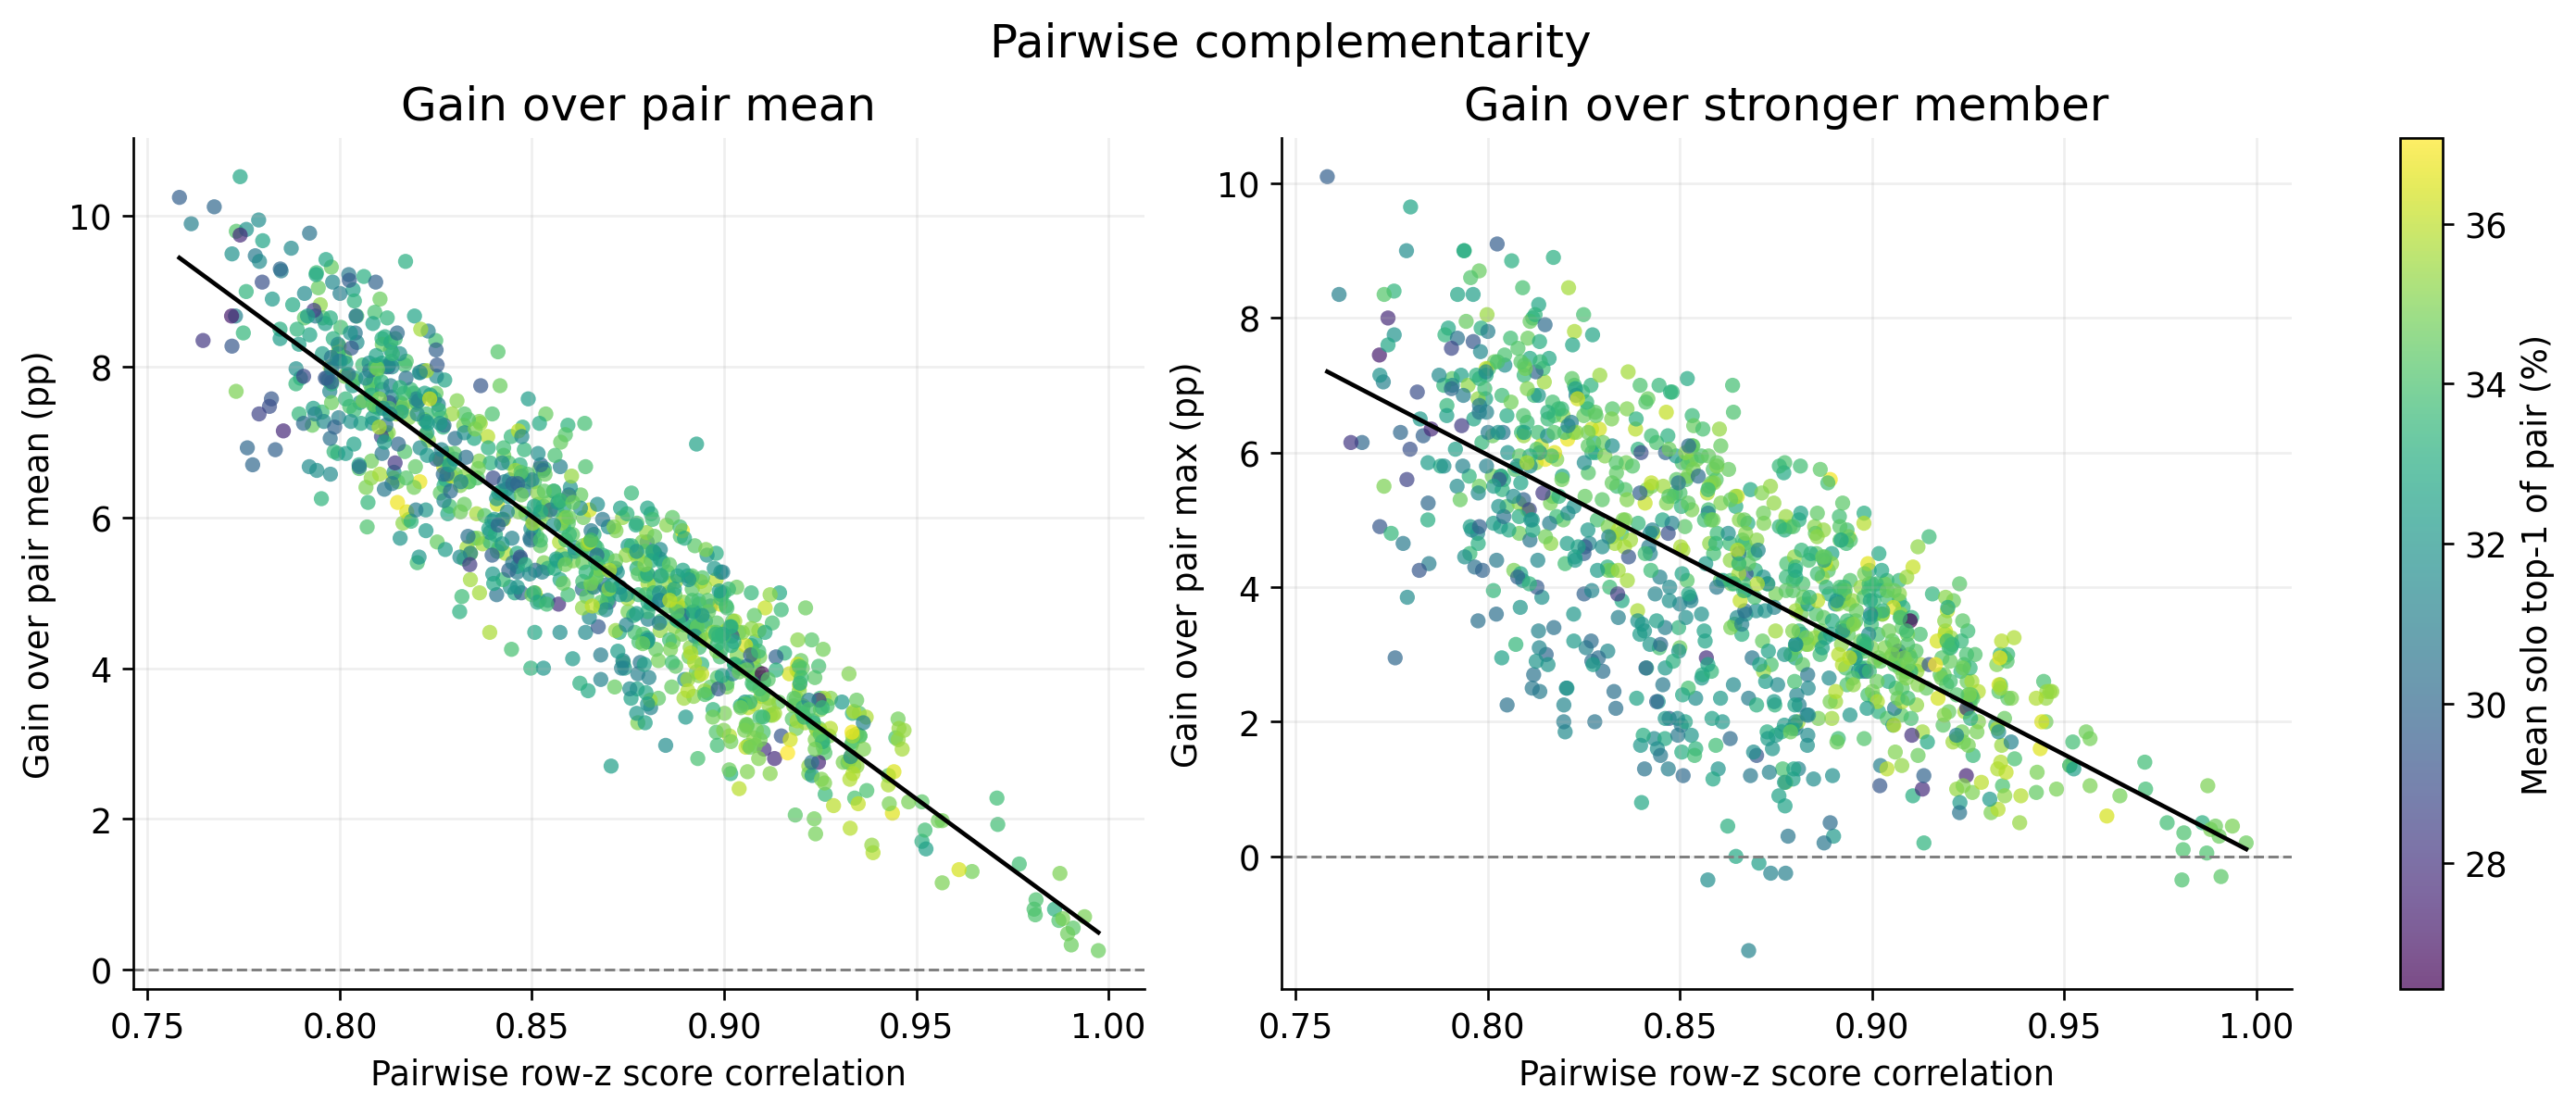
\includegraphics[width=0.94\textwidth,height=0.72\textheight,keepaspectratio]{pairwise_complementarity.png}

  \small For every single pair of model checkpoint available from our previous experiments
  (990 pairs), we show the ensembling gain over the mean and the max of the pair,
  as a function of the accuracy.
\end{frame}


\begin{frame}{A score-level error model}
  \small We model the \textbf{post-row-z retrieval score} of member $i$ as
  \[
    z_i(t,c)=\mu(t,c)+\eta(t,c)+\xi_i(t,c).
  \]

  \vspace{0.25em}
  \begin{center}
  \begin{tabular}{@{}cp{0.78\textwidth}@{}}
    \toprule
    Term & Interpretation \\
    \midrule
    $\mu$ & recoverable stimulus evidence: what accurate models should share \\
    $\eta$ & correlated error from the same EEG trial, artifacts, and LOSO shift \\
    $\xi_i$ & model-specific residual induced by architecture, seed, and optimization \\
    \bottomrule
  \end{tabular}
  \end{center}

  \vspace{0.35em}

  \takeaway{Members should agree on $\mu$; averaging can attenuate $\xi_i$, but not shared error $\eta$.}
\end{frame}

\section{From prediction to intervention}

\begin{frame}{Correlation is predictive, not yet causal}
  \begin{columns}[T,onlytextwidth]
    \column{0.47\textwidth}
      \textbf{Observed}
      \begin{itemize}
        \item lower score correlation $\leftrightarrow$ larger pair gain
        \item architecture changes move both at once
        \item member strength also changes
      \end{itemize}

    \column{0.47\textwidth}
      \textbf{Intervention}
      \begin{itemize}
        \item jointly train two members
        \item penalize correlated predictions
        \item sweep the penalty strength
      \end{itemize}
  \end{columns}

  \vspace{1.45em}
  \centering
  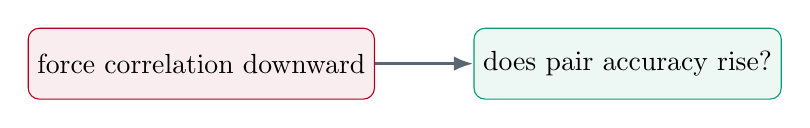
\begin{tikzpicture}[node distance=1.25cm,
      box/.style={draw,rounded corners,minimum width=3.5cm,minimum height=0.9cm,align=center},
      arr/.style={-{Latex[length=2.5mm]},very thick}]
    \node[box,draw=nbred,fill=nbred!7] (force) {force correlation downward};
    \node[box,draw=nbgreen,fill=nbgreen!7,right=of force] (gain) {does pair accuracy rise?};
    \draw[arr,draw=nbgray] (force) -- (gain);
  \end{tikzpicture}
\end{frame}

\begin{frame}{Artificial decorrelation}
  \small
  \begin{columns}[T,onlytextwidth]
    \column{0.49\textwidth}
      \centering
      \textbf{Twin TSConv}\\[-0.05em]
      \textit{two TSConv, different seeds}

      \vspace{0.45em}
      \begin{tabular}{@{}rrr@{}}
        \toprule
        $\lambda$ & corr. & pair \\
        \midrule
        0 & .956 & 37.10 \\
        .01 & .956 & 37.55 \\
        .05 & .957 & \textbf{38.25} \\
        .10 & .955 & 36.90 \\
        .50 & \textbf{.569} & 36.70 \\
        \bottomrule
      \end{tabular}

    \column{0.49\textwidth}
      \centering
      \textbf{ATM + TSConv}

      \vspace{1.55em}
      \begin{tabular}{@{}rrr@{}}
        \toprule
        $\lambda$ & corr. & pair \\
        \midrule
        0 & .850 & 40.15 \\
        .10 & .828 & 40.40 \\
        .25 & \textbf{.565} & \textbf{40.90} \\
        \bottomrule
      \end{tabular}
  \end{columns}

  \vspace{0.9em}
  \takeaway{The penalty can decorrelate scores by reshuffling low-ranked wrong candidates,
  without improving the correct-vs.-top-distractor margin that determines top-1.}
\end{frame}

\begin{frame}{Complementary-strength rescue}
  \begin{columns}[c,onlytextwidth]
    \column{0.54\textwidth}
      For each query, assign detached soft responsibility to the member with lower loss:
      \[
        r_m(q)=\operatorname{softmax}_m\!\left(-\ell_m(q)/\tau\right)
      \]
      \[
        \mathcal{L}=\mathcal{L}_A+\mathcal{L}_B
        +\gamma\sum_q\sum_m r_m(q)\,\ell_m(q).
      \]

    \column{0.42\textwidth}
      \begin{itemize}
        \item ordinary individual losses stay active
        \item specialize on queries already explained better
        \item target division of labor, not disagreement
      \end{itemize}
  \end{columns}

  \takeaway{The objective asks each member to rescue examples where it has comparative strength.}
\end{frame}

\begin{frame}{Intervention trajectories}
  \centering
  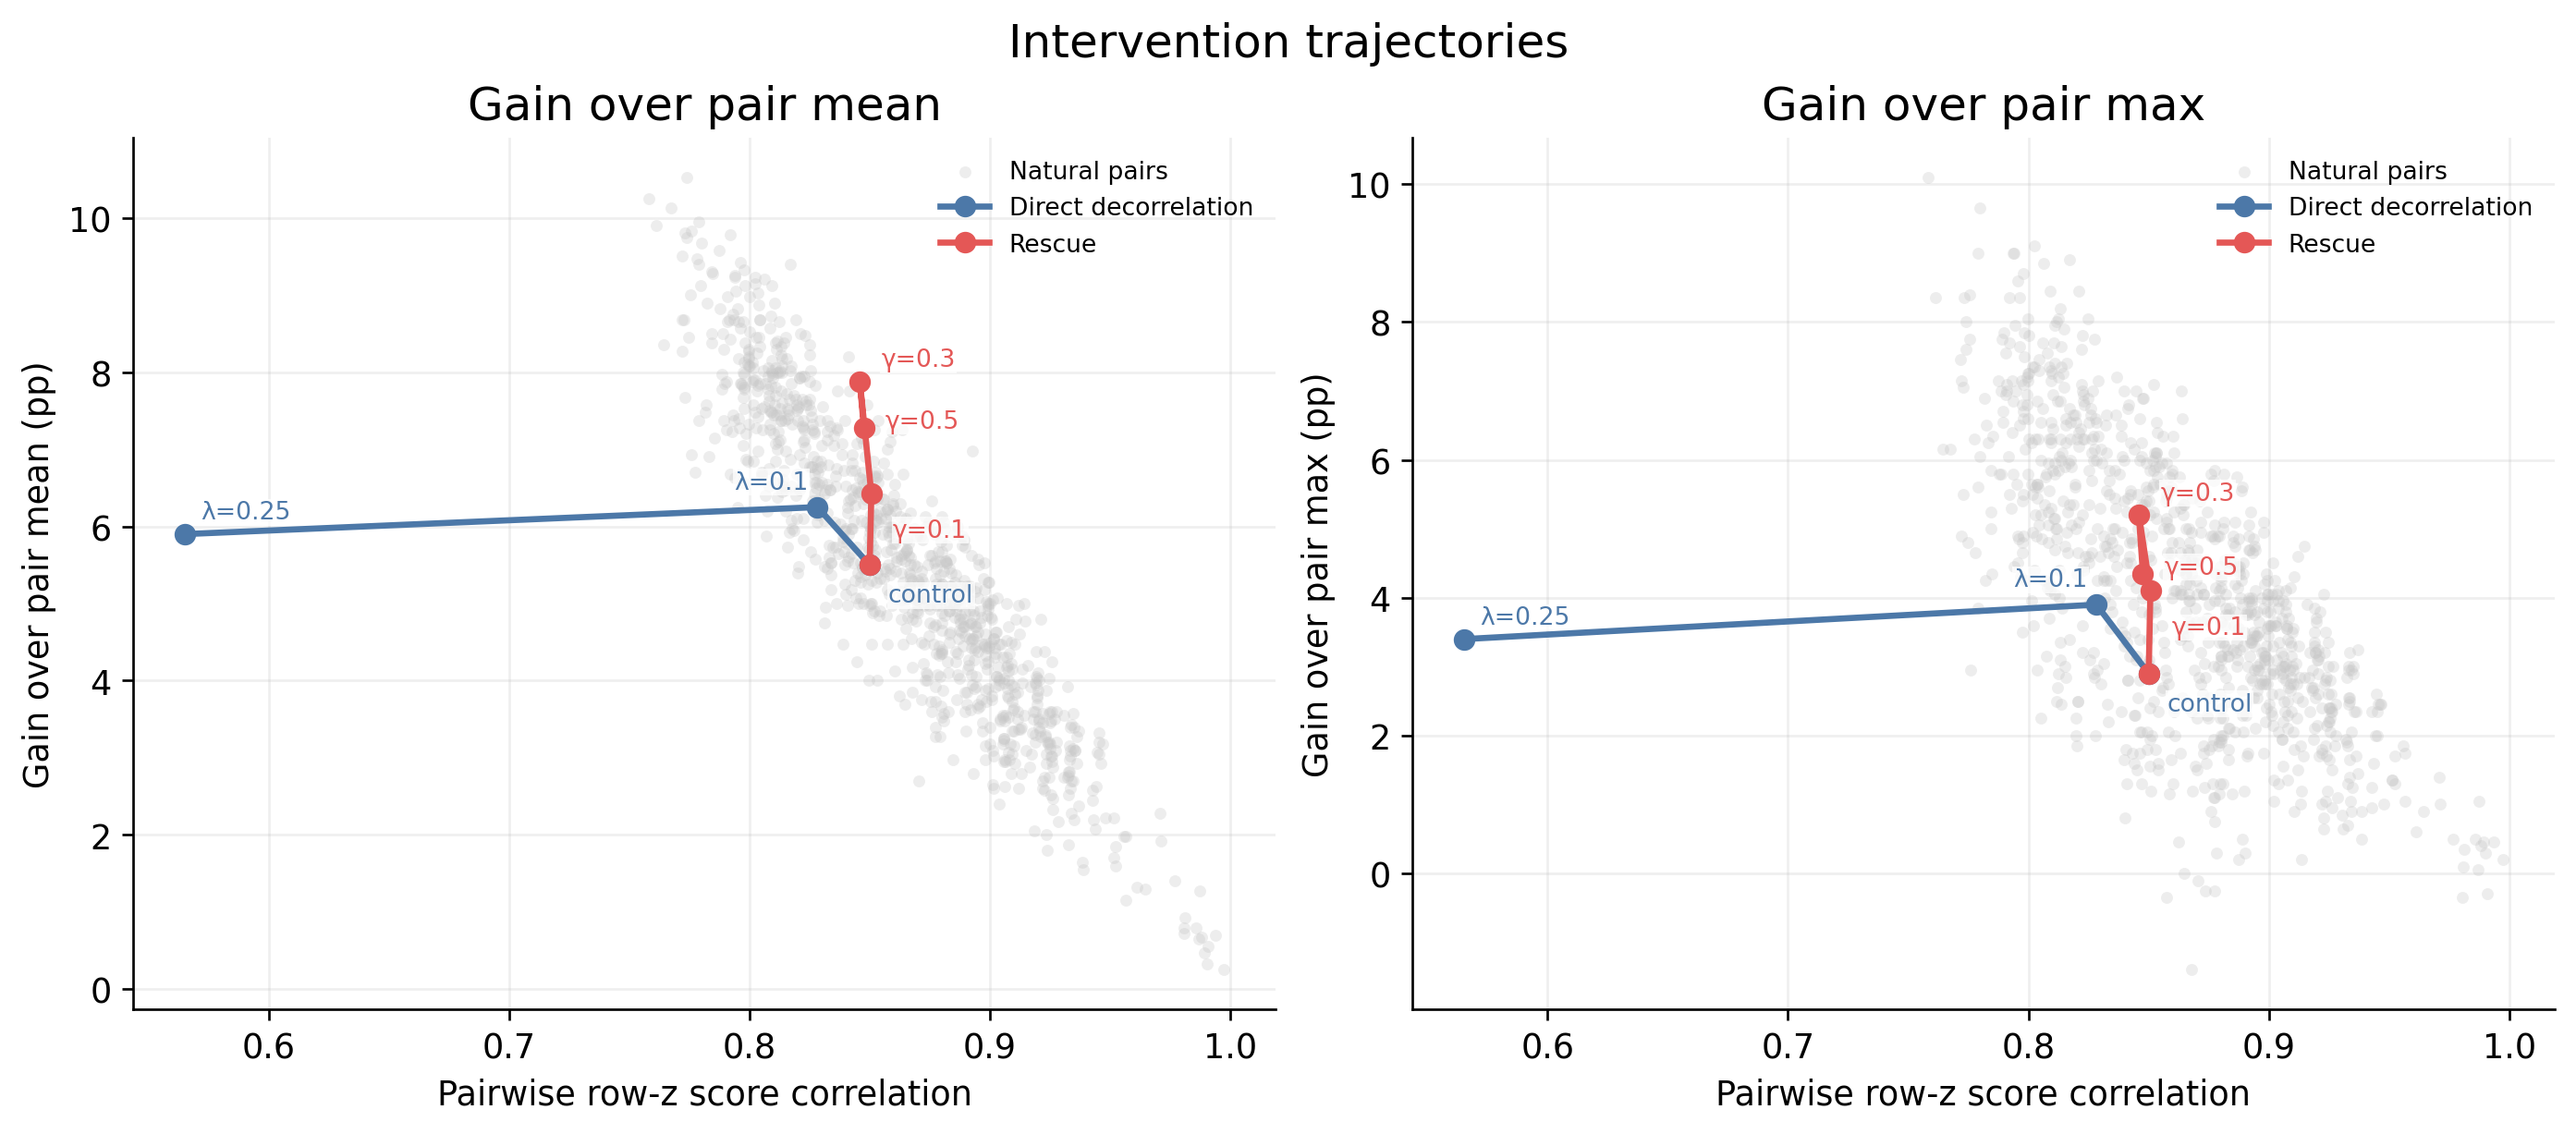
\includegraphics[width=0.92\textwidth,height=0.77\textheight,keepaspectratio]{intervention_trajectories.png}
\end{frame}

\begin{frame}{Complementary-strength rescue results}
  \centering
  \small
  \begin{tabular}{@{}rrrr@{}}
    \toprule
    $\gamma$ & Pair top-1 & $\Delta$ vs. control & Score corr. \\
    \midrule
    0 & 40.15 & --- & .850 \\
    .10 & 40.75 & +0.60 & .851 \\
    .30 & \textbf{41.90} & \textbf{+1.75} & .846 \\
    .50 & 41.65 & +1.50 & .848 \\
    \bottomrule
  \end{tabular}

  \vspace{1.0em}
  \takeaway{$\gamma=.30$ improves pair accuracy by $1.75$ points while score correlation stays nearly unchanged.}
\end{frame}

\section{Validation}

\begin{frame}{ValCon outperforms LOSO-subject validation}
  \centering
  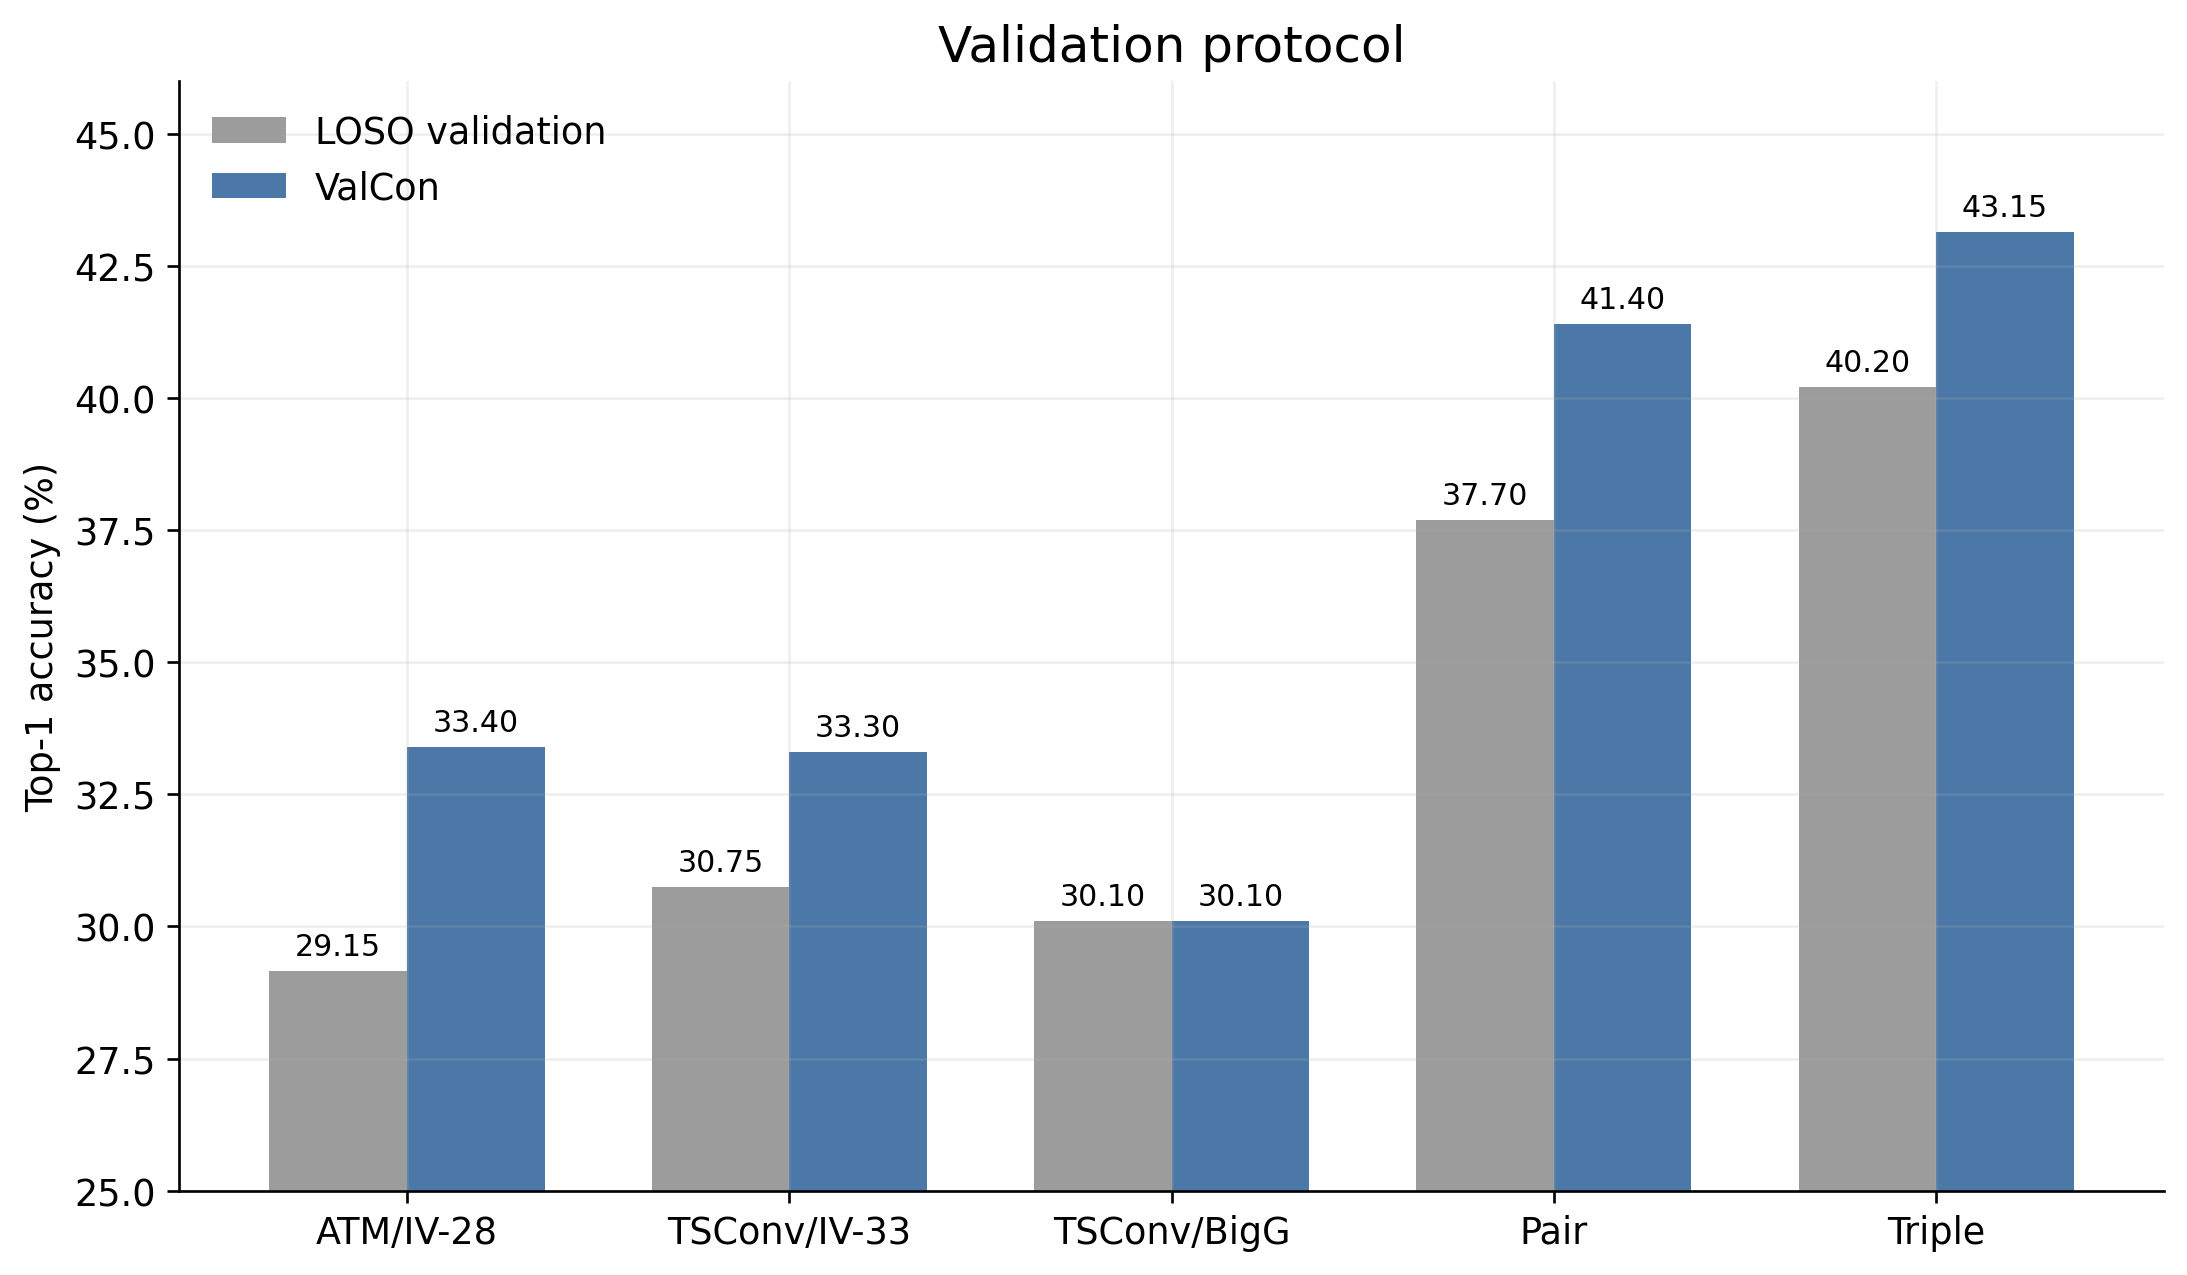
\includegraphics[width=0.89\textwidth,height=0.72\textheight,keepaspectratio]{validation_protocol.png}

  \takeaway{Mean solo: $+2.27$ points; pair: $+3.70$; triple: $+2.95$.}
\end{frame}

\begin{frame}{ValCon ensemble scaling}
  \centering
  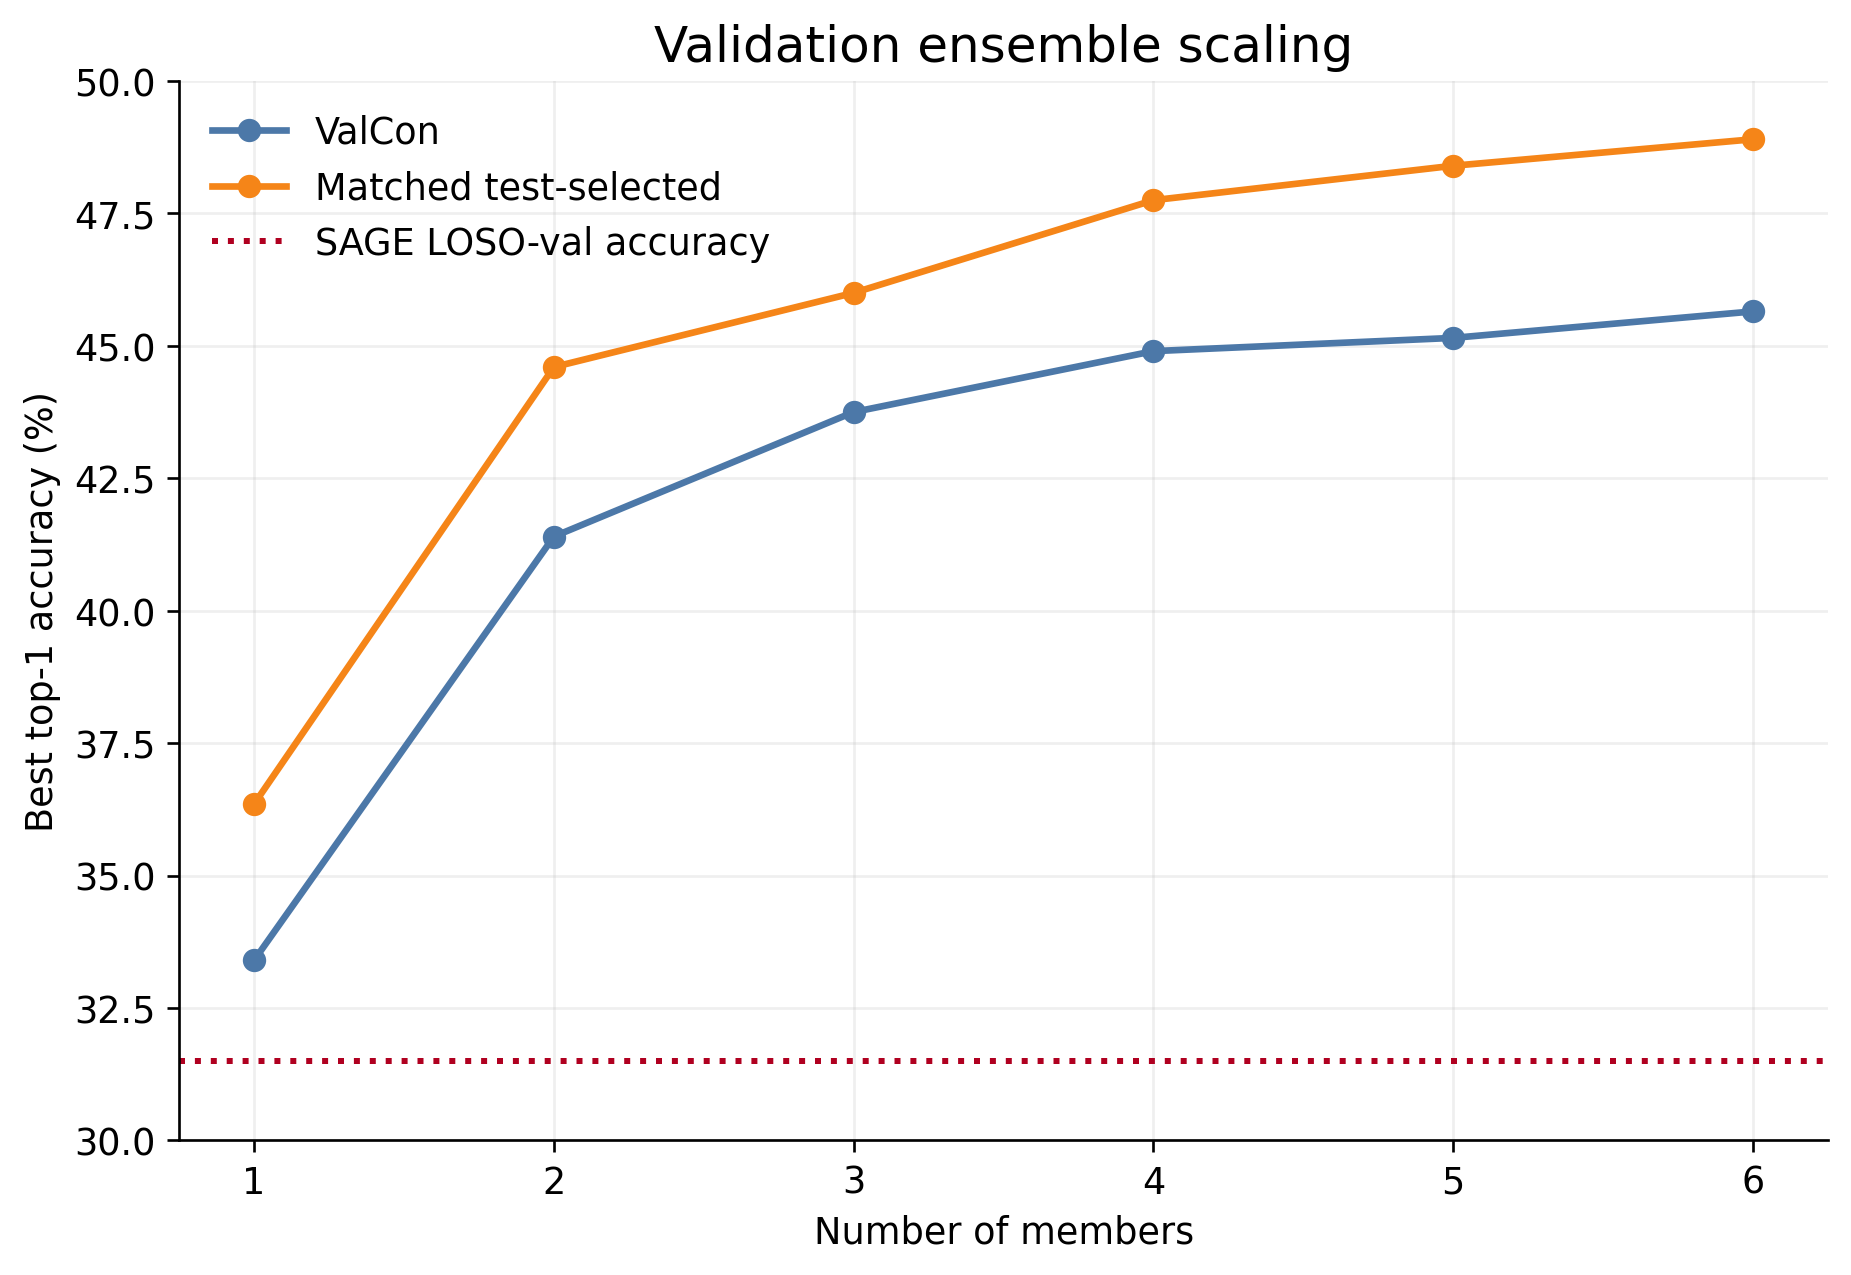
\includegraphics[width=0.90\textwidth,height=0.71\textheight,keepaspectratio]{validation_ensemble_scaling.png}

  \takeaway{$45.65\pct$ at $k=6$ under ValCon; matched test selection is $48.90\pct$.}
\end{frame}

\begin{frame}{Rescue by selection protocol}
  \vspace{4pt}
  \begin{center}
  \small
  \begin{tabular}{@{}lrrrr@{}}
    \toprule
    Selection & $\gamma$ & Pair top-1 & $\Delta$ vs. control & Score corr. \\
    \midrule
    Test-selected & 0 & 40.15 & --- & .850 \\
    Test-selected & .10 & 40.75 & +0.60 & .851 \\
    Test-selected & .30 & \textbf{41.90} & \textbf{+1.75} & .846 \\
    Test-selected & .50 & 41.65 & +1.50 & .848 \\
    \midrule
    ValCon & 0 & 38.10 & --- & .832 \\
    ValCon & .10 & \textbf{38.55} & +0.45 & .830 \\
    ValCon & .30 & 37.75 & $-0.35$ & .834 \\
    ValCon & .50 & 37.60 & $-0.50$ & .826 \\
    \bottomrule
  \end{tabular}
  \end{center}

  \takeaway{The $\gamma=.30$ test-selected gain does not reproduce under ValCon.}
\end{frame}

\section{Conclusion}

\begin{frame}{Takeaways}
  \begin{center}
  \begin{tabular}{@{}cl@{}}
    \toprule
    1 & Encoder diversity produces the dominant ensemble gain. \\
    2 & Natural decorrelation predicts complementarity; forcing it creates junk diversity. \\
    3 & Rescue targets usable evidence, but its test-selected gain fails under ValCon. \\
    \bottomrule
  \end{tabular}
  \end{center}

  \vspace{0.8em}
  \takeaway{Strong members $+$ complementary correct evidence $+$ compatible confidence.}
\end{frame}

\begin{frame}{References}
  \small
  \begin{thebibliography}{9}
    \bibitem{Krogh1995} A. Krogh and J. Vedelsby.
      \newblock Neural network ensembles, cross validation, and active learning. 1995.
    \bibitem{Ueda1996} N. Ueda and R. Nakano.
      \newblock Generalization error of ensemble estimators. 1996.
    \bibitem{Liu1999} Y. Liu and X. Yao.
      \newblock Ensemble learning via negative correlation. 1999.
    \bibitem{Fort2019} S. Fort, H. Hu, and B. Lakshminarayanan.
      \newblock Deep ensembles: A loss landscape perspective. 2019.
    \bibitem{Jeffares2023} A. Jeffares et al.
      \newblock Joint training of deep ensembles fails due to learner collusion. 2023.
  \end{thebibliography}
\end{frame}

\end{document}
